\documentclass[journal]{IEEEtran}
% *** CITATION PACKAGES ***
\usepackage{cite}
\usepackage{graphicx}
% *** GRAPHICS RELATED PACKAGES ***
%
\ifCLASSINFOpdf
  % \usepackage[pdftex]{graphicx}
  % declare the path(s) where your graphic files are
  % \graphicspath{{../pdf/}{../jpeg/}}
  % and their extensions so you won't have to specify these with
  % every instance of \includegraphics
  % \DeclareGraphicsExtensions{.pdf,.jpeg,.png}
\else
  % or other class option (dvipsone, dvipdf, if not using dvips). graphicx
  % will default to the driver specified in the system graphics.cfg if no
  % driver is specified.
  % \usepackage[dvips]{graphicx}
  % declare the path(s) where your graphic files are
  % \graphicspath{{../eps/}}
  % and their extensions so you won't have to specify these with
  % every instance of \includegraphics
  % \DeclareGraphicsExtensions{.eps}
\fi


\hyphenation{op-tical net-works semi-conduc-tor}


\begin{document}

\title{Smart File system}

\author{Fabian Spie\ss, Max Mustermann}
        
% make the title area
\maketitle


\begin{abstract}
%\boldmath
The abstract goes here.
\end{abstract}

\IEEEpeerreviewmaketitle



\section{Introduction}
\IEEEPARstart{T}{his} demo file is intended to serve as a ``starter file''
for IEEE journal papers produced under \LaTeX\ using
IEEEtran.cls version 1.7 and later.
I wish you the best of success.

\hfill mds
 
\hfill January 11, 2007

\section{The Systemarchitecture}

\IEEEPARstart{B}{ased} on project restrictions and own decisions there was a hardware and software mixed test system created. This chapter will give a short introduction about how all the system parts are connected to each other. Detailed description about single parts will follow later.

\subsection{Hardware Setup}

Given by the project initiator, the Institute for Complex and Distributed IT systems of TU Berlin (CIT), some hardware components were directly defined as prerequisites.

\begin{enumerate}

\item One powerful machine with high power usage of around 350W placed in tubit data centre (TU Berlin), later called by name \textit{Asok05}.

\item One energy-saving \textit{office pc} attached to TU network inside a staff office with lower bandwidth and power drain of 75W in idle mode.

\item Two energy meters by type \textit{EGM-PWM-LAN} of the brand \textit{Energenie} which were used to measure the current drain of \textit{Asok05} and \textit{office pc}.

\item For running services which should not influence the power usage measured by the energy meters, a virtual machine, placed in the tubit data centre was prepared to be used, too.

\end{enumerate}

\todo{add some machine details (storage/bandwidth)}

\subsection{Software Setup}

The partly introduced software systems were used by team decisions described in the following chapters.

\begin{enumerate}

\item As distributed file system Apache Haddop\textsuperscript{\textregistered} (HDFS) was used. The access to the filesystem is be done using a terminal, a web client or a client as provided by Filesystem in Userspace (FUSE). HDFS consists of two main parts, the namenode which organises the filesystem structural view, and datanodes which store and replicate the data as blocks.

\item To measure network traffic, all data were sent through a virtual network. A combination of Floodlight as controller and an Open vSwitch was used. 

\item For monitoring user actions in the filesystem and on the software defined network a zabbix server was used. This service collects data from clients which are running a zabbix agent.

\item To analyze the changes in energy consumption produced by user activities the power consumption of \textit{office pc} and \textit{Asok05} were measured.

\item By evaluating the monitored data we are finally able to create a  report which informs about the power consumption for the whole system and for a single user. This service was implemented as web service on \todo{where is it running actually?}.

\end{enumerate}

\subsection{Services Setup}

As an overview the distribution of services used in project are given in table~\ref{tab:services}. Mainly the virtual machine was used for common services, while the \textit{office pc} and \textit{Asok05} were used to deliver data to the client machine over the sdn.

\todo{add report web service to table}

\begin{table}[b]
	\centering
	\caption{Services and machines overview used in project. }
	\begin{tabular}{|l|l|l|l|l|}
		\hline \rule[-2ex]{0pt}{5.5ex} \textbf{Client PC} & \textbf{Office PC} & \textbf{Virtual Machine} & \textbf{Asok05} \\ 
		\hline \rule[-2ex]{0pt}{5.5ex} Hadoop client & Hadoop data node & Hadoop name node & Hadoop data node \\ 
		       \rule[-2ex]{0pt}{5.5ex}  & Energy meter & Zabbix server & Energy meter \\ 
		       \rule[-2ex]{0pt}{5.5ex}  & Zabbix agent & Zabbix agent & Zabbix agent \\ 
		       \rule[-2ex]{0pt}{5.5ex}  &  &  & Floodlight \\ 
		       \rule[-2ex]{0pt}{5.5ex}  &  &  & Open vSwitch \\ 
		       \rule[-2ex]{0pt}{5.5ex}  &  &  & Energy data agent \\ 
		\hline 
	\end{tabular}
	\label{tab:services}
\end{table}


\section{Filesystem}

\subsection{Motivation}

To offer multiple users and applications a high available access on large filesystems there are different solutions known. Files can be stored on local filesystems (fs), may be shared using a network attached storage (nas)  or using a storage area network (san). for sharing storage in datacenters a san actually is a common used solution. they offer a redundant hardware setup on different locations using SCSI on FibreChannel or iSCSI over IP.
There are less limitations on the given ressource power and data transmission speed but a manufacturer will connect a customer to original equipment which limits a customer through expansion costs.

a possible solution for this case could be a cluster filesystem that consists of a lot of heterogeneous (smaller) computer systems. such a system should share computation between all nodes and give a lot of configurable options for keep redundant copies of files and offer fast delivery of files out of the network based on the number of nodes in that system.

by holding a software based virtual filesystem it should be possible to react on new desires of customers like on filesize, number of files, available bandwidth. in opposite by having to many nodes the computation power is much to high and expensive for the given storage amount.  otherwise there will be a lot of work for keeping all the systems up to date. 

we were interested in how to reduce costs by providing different customer plans to fulfil a given quality-of-service (QoS) aggreement by starting to separating into a expensive speed oriented and slower/cheaper plan. the costs should be 

\subsection{comparison of common cluster file systems}

\begin{itemize}
\item was ist ein verteiltes dateisystem
\item auswahl/unterschiedliche ansätze, vergleich, begründung der auswahl
\item ziele
\end{itemize}

\subsection{System setup}

wdh einleitung, ergänzungen sofern nicht später beschrieben:

\begin{itemize}
\item verbindung zu sdn
\item verbindung zu zabbix
\end{itemize}

\section{Extensions written}

\subsubsection{server selection for downloading files}

\subsubsection{static selection}

hintergrund, vermutungen, implementierung, test, auswertung

\subsubsection{dynamic selection}

hintergrund, vermutungen, implementierung, test, auswertung

\subsection{Client connection}
\subsubsection{Terminal}
\subsubsection{FUSE}

\subsection{reached goals}
gesamte auswertung





%\IEEEPARstart{J}{ust} start typing your Text here... Then compile the main document!


\section{Software Defined Network}
In the last years, the concept of \textit{Software Defined Networking(SDN)} got more and more important. The idea of this concept was created by the introduction of the \textit{OpenFlow} protocol in 2008\cite{Mc2008}. This protocol provides a secure communication between switches of a network and some other part of software. Furthermore entries of forwarding tables of these switches can be dynamically modified by this protocol. This allows the ability to change network flows at any time to get an optimal behaviour for special situations. This is basically the idea of \textit{Software Defined Networking}, which is currently promoted and propagated by the \textit{Open Networking Foundation}\cite{onf}. 
\subsection{Overview}
A Software Defined Network contains two important parts. A network with OpenFlow supported switches and a controller. A controller denotes the part of software which controls the behavior of the network at any time by using OpenFlow. In normal networks each switch is its own controller. When a connection starts the switch takes a lookup in its forwarding table to forward the packages. If there is no entry it performs some routing algorithm to get this entry. The problem is that there is nothing which has a view on the whole network. For example if a device has a failure it will take time until each connection node is aware of it. Or maybe if one path of the network is overloaded, it might be faster to send packages via another path. This is a feature, a normal network device can not easily provide. In an emergency case where i.e. a live stream of security cameras needs a higher priority than anything else, a SDN could dynamically provide that in seconds. It works, because a controller of a Software Defined Network sees the network as a graph. It is in a permanent contact with all devices to detect failures. It can get the workload of each switch and can route some communications over other nodes, if a device is overloaded. So the controller can be denoted as the brain of a network and the network nodes as the nerves which follow the orders of the brain. If a new network flow starts, the switch contacts via OpenFlow the controller. The controller decides what to do and sends to the switch a flow table entry. A flow table is the forwarding table in an OpenFlow switch. If the flow finishes, the OpenFlow switch deletes this entry from its flow table. So there is never an uncontrolled flow in the network. The concept of a SDN is visualized in figure \ref{sdn}.\\
\begin{figure}[ht]
\centering
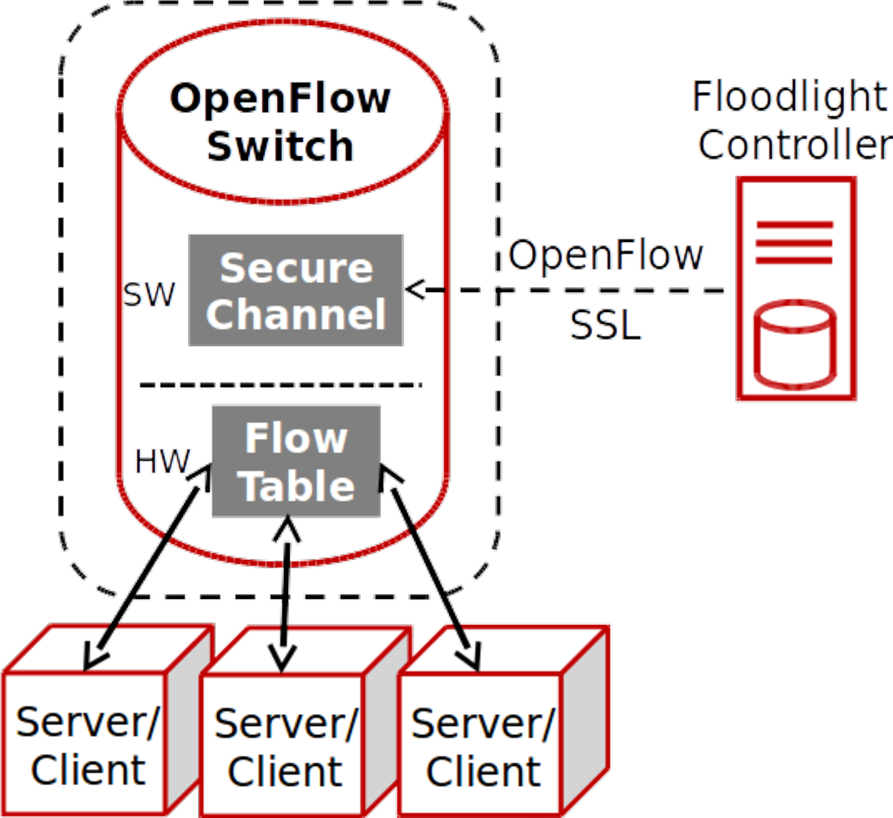
\includegraphics[width=0.25\textwidth]{img/sdn} 

\caption{SDN with Floodlight and Open vSwitch}
\label{sdn}
\end{figure}
 

\subsection{System Setup}
To provide a SDN in the smart Filesystem, the network is organized by the SDN controller Floodlight\cite{flood}. Floodlight is an open source SDN controller, which is written in Java. The fact, that it is written in Java, makes it easy to set it up on many different machines. Floodlight comes with an OpenFlow implementation for virtual switches, as well as physical switches. Moreover it has a lot of additional features. For example features to modify OpenFlow switches or a shortest path routing within a network. Furthermore it is easy to extend Floodlight by using provided interfaces or adding new basic features as so called \textit{Modules}. All in all Floodlight allows a quick start in programming a SDN.

As counterpart to the controller, the SDN needs an OpenFlow switch. As told, OpenFlow is a very new protocol. In the moment there are companies like \textit{HP}, \textit{Arista}, \textit{Brocade} or \textit{Dell} , which build switches with OpenFlow support. Besides that, these companies designing switches for large networks where one switch is expensive. A good alternative to physical switches is the \textit{Open vSwitch} project\cite{ovs2}. With this project it is possible to set up a virtual switch with OpenFlow support on a system, which just behaves like a normal switch. This switch can be controlled by Floodlight very easily. A small disadvantage is, that Open vSwitch is currently supporting OpenFlow 1.0\cite{ovs}, but the latest version is OpenFlow 1.4\cite{ofspec4}. However, version 1.0 supports a lot of features and is sufficient for the needs of the Smart Filesystem.
This Open vSwitch connects all parts of the Smart Filesystem by using OpenVPN connections.     
   
\subsection{Usage in the Smart Filesystem}\label{usage}
In the Smart Filesystem we use Software Defined Networking to measure the file transactions of users within the system. With OpenFlow 1.0, the controller is able to request for flow statistics \cite[P. 31]{ofspec}. These flow statistics contain information such as IP adresses, MAC adresses, used TCP ports, transfered bytes and running time of the flow. With this information the controller is able to tell, that user $u$ with IP $i$ and port $p$ has transferred $x$ bytes in $s$ seconds with an average bandwidth of $x/s$. The identification of the connection with IP and port allows, that more than one user from the same system can use the file system at the same time.

 Of course there are more flows in the file system than just file transfers. But all file transfer flows contain the port $p=50010$ and the IP from one of the datanodes in the HDFS. So if there is a connection, where source or destination is IP $i$ and port $p$, than this is a connection the controller is interested in.
 
 When the controller finds a flow like this, it calculates the bandwidth every five seconds and sends it to the monitoring system. With this data the admins of the file system are able to oversee all transactions and to calculate a very specific power usage for each user. 
 
 \subsection{Implementation and Connection Establishing}               

To establish a connection for file transferring, there are four parts inside the network which need to be done. The first step is shown in figure \ref{nn}.
 
\begin{figure}[htp]
\centering
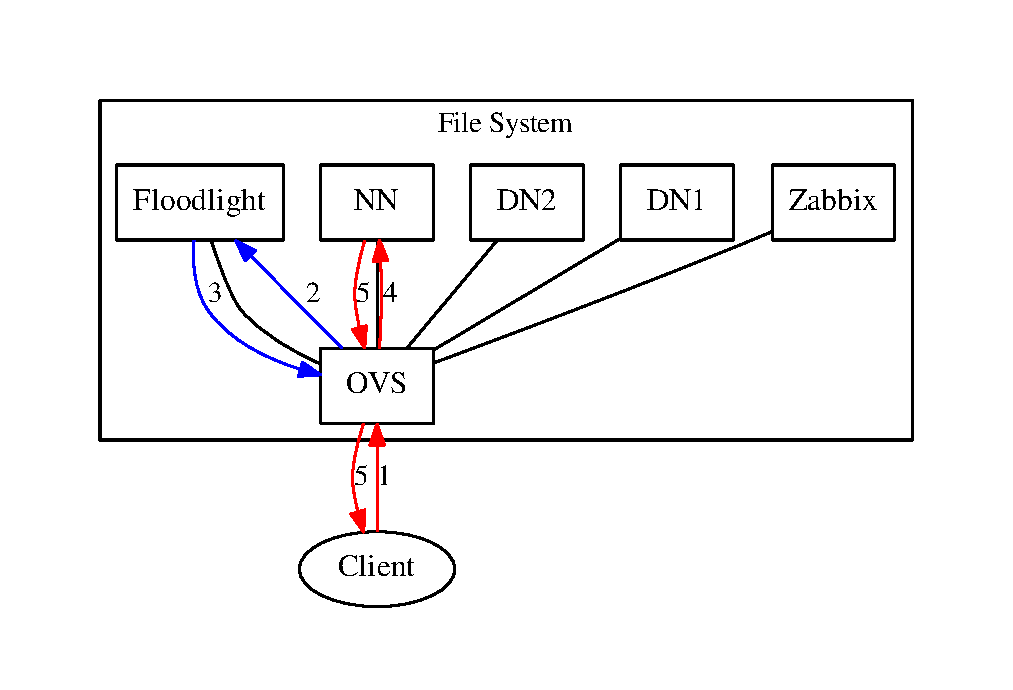
\includegraphics[width=0.45\textwidth]{img/connectionToNamenode} 
\caption{Part 1: A user tries to connect to the Namenode}
\label{nn}
\end{figure}

Figure \ref{nn} shows the internal file system and a client who wants to start a file transfer. The dotted edges denotes client/system interactions and the dashed edges are interactions within the system. The bold edges denotes the openVpn connections of the system.

In step 1 of the figure the client wants to start a file transfer. So the first thing to do is to send a connection request to the system. This request goes firstly to the Open vSwitch(OVS). The switch does not know, where to forward the connection because there is no flow table entry. So the switch asks Floodlight, shown in step 2. In step 3 Floodlight computes the path in the network and sends the flow entry back to the switch. Before a file transfer can start, the Namenode(NN) has to decide on which server the client can connect. So the request goes further to the Namenode, shown in step 4. The Namenode decides for one server and sends these information in step 5 back to the client. Now the client is ready to connect with the Datanode. This interaction is shown in figure \ref{dn}.

\begin{figure}[htp]
\centering
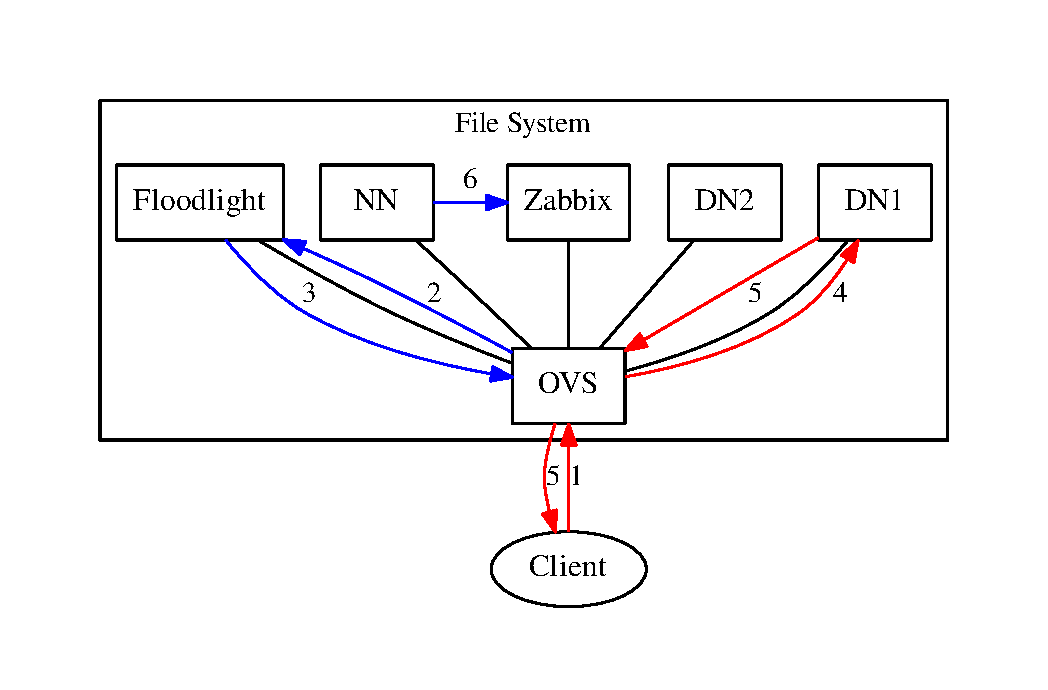
\includegraphics[width=0.45\textwidth]{img/connectionToDatanode} 
\caption{Part 2: Starting connection to the Datanode to begin a file transfer}
\label{dn}
\end{figure}     

In the second part, the client is now really able to start the file transfer and tries to open the connection. Again this connection request stops at the switch, which needs to find out where to forward this request. So the steps 1 till 3 are the same as in the first part. After that, the flow table of the switch contains an entry for this connection request and it can forward it to i.e. Datanode 1(DN1). This is shown in step 4. In step 5 the Datanode answers the request and Client and Datanode 1 start the file transfer. 

Important in the second part is step 6. The Namenode not only decides to which Datanode the connection goes, but also it checks if the client is a registered user. If he is, the Namenode will send the username and the current IP with port of the user to the monitoring system "Zabbix". Why it does that, is described in the third part, which is shown in figure \ref{wc}.    

\begin{figure}[htp]
\centering
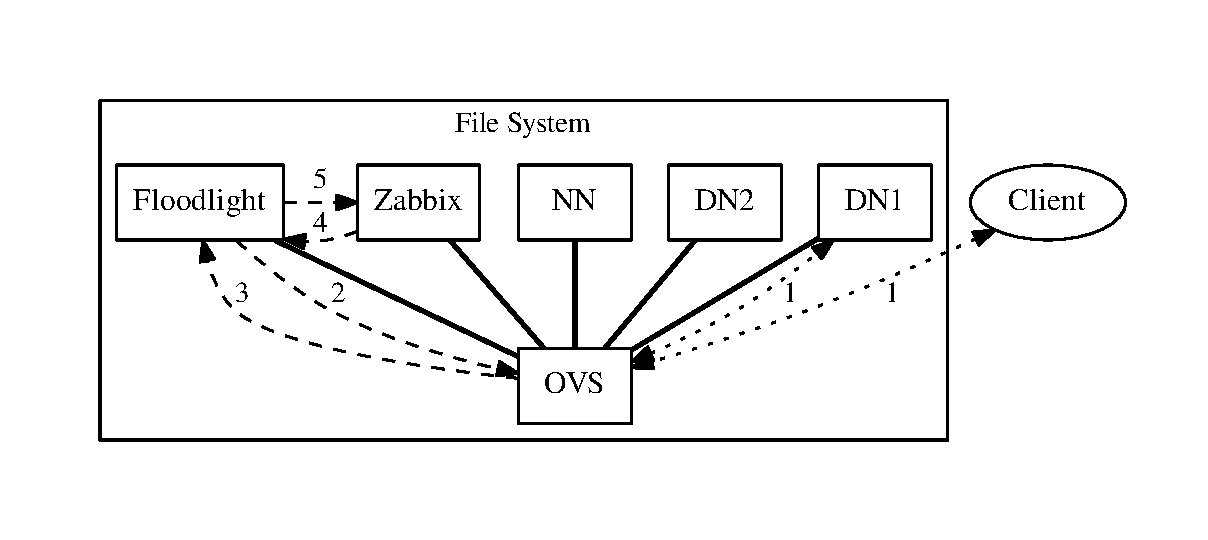
\includegraphics[width=0.45\textwidth]{img/whileConnection} 
\caption{Part 3: While the user is transferring files from or to the Datanode}
\label{wc}
\end{figure}

The figure of part three shows the interactions while a file transfer between client and DN1 is running. Every five seconds Floodlight asks the Open vSwitch for statistics of each entry. Floodlight can do this, because OpenFlow provides a \textit{Read State Message}\cite[p. 30]{ofspec}. With this message, Floodlight gets all the statistics of each flow, which were mention in subsection \ref{usage}. This statistic request is shown in steps two and three. In the moment, there should be two entries for the file transfer. One for uploading and one for downloading. In each case the source/destination is the IP of DN1 with port $50010$. So Floodlight detects, that these are interesting connections and computes the current bandwidth. One problem is, that Floodlight cannot say, which user is using this connection. It only has the IP and port of the user. To solve this problem, the Namenode has sent in the last part the username with corresponding address and port to Zabbix. Now Floodlight can ask Zabbix by using the \textit{Zabbix-API-Client} which user has the IP and port of the connection. The Zabbix-API-Client is an interface to communicate with Zabbix which was build within the scope of this work and will be explained later in this paper. If Zabbix has such an entry, it will send the username to Floodlight, shown in step 4. Now Floodlight can compute the bandwidth for each user and sends it back to Zabbix. This is shown in step 5.

With this procedure, the file system is able to create a precise bandwidth usage for each user every five seconds. After Floodlight has got the connection information from Zabbix, it hashes them to avoid more unnecessary requests. To mention is, that these statistic requests are not bound to the five seconds. This was just a decision to create not too much traffic.

To be sure to get the statistics of the complete flow, the system needs a fourth part, see figure \ref{cc}.  

\begin{figure}[htp]
\centering
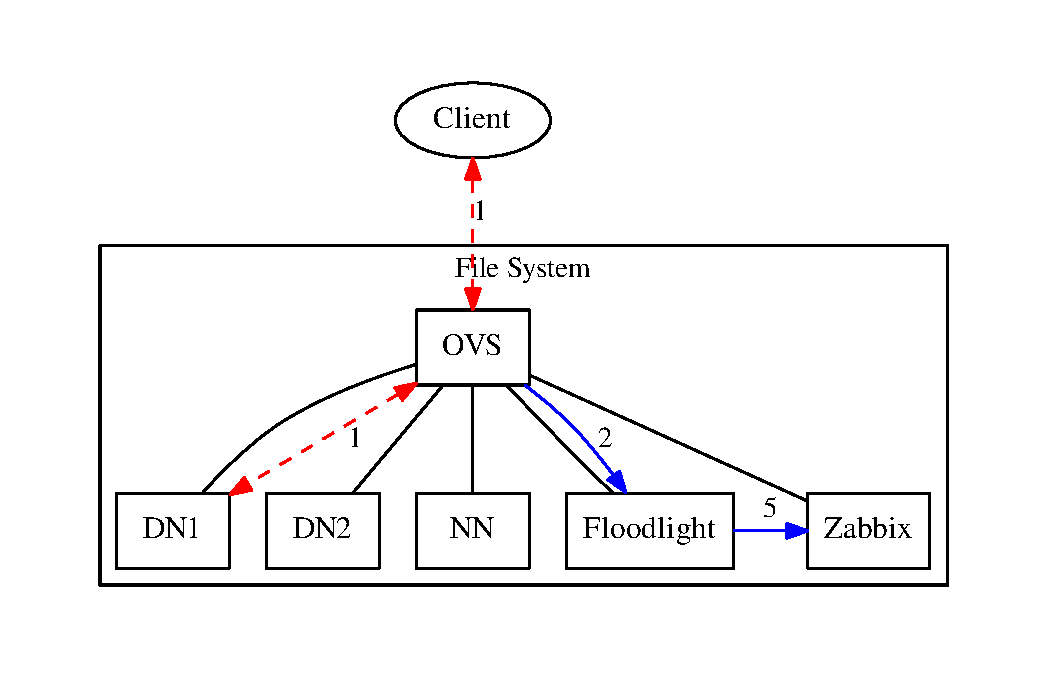
\includegraphics[width=0.45\textwidth]{img/closeConnection} 
\caption{Part 4: Closing connection after file transfer}
\label{cc}
\end{figure}

The last part shows, what to do if a file transfer has finished. The dashed edges of figure \ref{cc} symbols that the connection just closed. When the flow table entry was created it got an \textit{idle timeout}\cite[p. 11]{ofspec}. When there is no data flow any more, the switch waits this idle timeout(here 5 seconds) until it removes the entry from the flow table. Before it removes the entry, it sends a \textit{Flow-Remove-Message}\cite[p. 37]{ofspec} to Floodlight. These messages are just an option which can be set when the entry is created. With this message, Floodlight not only knows that it can remove the flow from its data structures, but also floodlight gets one last time all statistics of this flow. This message is shown in step 4. So Floodlight can compute the bandwidth for the user again and sends it in step 5 to Zabbix. After that it removes the connection information and user name from the data structures and the flow monitoring is done.

\subsection{Additional Information}

Software Defined Networking is an innovation which contains a lot new and interesting features for future networks. The ability to dynamically modifying and reprogramming a network allows a much further improvement of the QoS aspect. But also for the File System it can bring a lot of advantages.

The problem is that the main concern of SDN is to reprogram a network. In our test system there is only one Open vSwitch. So there are not many possibilities to do that. In larger file systems it could be conceivable to transfer all functions of the Namenode to the controller of the SDN. This could save the energy for one device and would be more compact. Moreover, because the controller is always aware of the traffic in the network, it could check if there are datanodes which has not been used in the last time. If there are some, the controller could set to a sleeping mode until there are new traffic for these datanodes. This could save a lot of energy considering that the Asok05 datanode uses $400\ W$ in idle time. It is also possible to modify paths, if a user uses a special profile to get a faster connection of switches or if the user wants to change the profile while doing file transfer. Changing paths can also help for reducing energy costs. The really big switch \textit{HP 12518 AC Switch Chassis} has a maximum power rating of $10700\ W$\cite{hp}. Of course this is a very big switch and this power usage is only if all components are $100\%$ in usage. But it shows that network nodes should be factored into the goal of reducing energy usage. In the end it still needs to be calculated in special situations, if it is better to use just a few nodes or if it is more energy efficient to spread the traffic over the whole network. 

To conclude, in our test system we are able to separate traffic, such that each user can exactly see how much traffic he or she produced. Moreover the file system can collect a lot of statistic values. But to use this values and the whole power of SDN in the way to provide more energy efficiency, it would need a larger test system.  


\section{Zabbix}

\subsection{Zabbix}

\subsubsection{Motivation}
	The necessity for administrative tasks on great number of computers can be tedious and time consuming without any means of automation or help. As the information on every single computer or system needed to be done one after another separately from each other as the administered systems could vary greatly in both the used hardware and the software which was installed on them. Furthermore with current distributed systems which could span the globe it is further difficult to administer these since there is now also a great distance for the administrator to travel to actually access the systems. Thus arose a need for a program which would support the surveillance and to a certain degree the control of a collection of systems. Such a program should grant the administrator a centralized access to view the status of all necessary systems. These programs were called monitors.
\subsubsection{Monitor}
	The key component of this project is the monitor, which is responsible for the surveillance of the projects systems. A monitors job is the surveillance and data gathering of systems or processes and storage of any acquired data for further analysis later on. Beyond that monitors also are tasked with presenting their data in a comprehensible way to its user. Thus monitors have to provide a means to visualize any of their data. Since a administrative user cannot be around all the time, the monitor has to be able to act on its own by surveying the received data and act or send out alerts should the received values exceed given thresholds. From its tasks its vivid that a monitor is not just a simple watcher.\cite{zab1}
\subsubsection{Zabbix}
	\textit{Zabbix} is such a monitor and thus is tasked with the job of surveying systems for administrative controlling. The surveyed systems can be whole computers, virtual machines within a computing cloud or even network devices. \textit{Zabbix} is an Open Source monitor licensed under the \textit{GPL} license and written in programming language\ C\ and thus compiled for a great variety of different operating systems to ensure optimal functionality. It is so to prevent \textit{Zabbix} from consuming resources which are necessary for other tasks on the surveyed systems, as\ C\ programs compiled for specific systems are specifically tuned for them. For that reason \textit{Zabbix} splits its functionality into two. The \textit{Zabbix server} which is tasked with accumulating all the acquired information and data and the \textit{Zabbix agent}, which other than the \textit{Zabbix server} is installed directly on the surveyed system, is tasked with gathering information for the server. \textit{Zabbix server} can receive the input from a great number of agents and thus it is a centralized single monitor service. The \textit{Zabbix server} stores all the acquired data in its own database, which can be a SQL database, for example \textit{MySQL} or \textit{PostgreSQL}. For the ease of access for the gathered data and also for the easier configuration the \textit{Zabbix server} has a web frontend. The web frontend gives a lot of possibilities to configure and view different data or the surveyed systems and to group and categorize the systems themselves too. But the most important functionality of the \textit{Zabbix web frontend} is its capability to visualize the stored data values in graphs for easier understandings and readability by its users. From these graphs the user can see the times when the items, so called data representation types within \textit{Zabbix}, took on which values and thus allow seeing their trending. These items created within the \textit{Zabbix server} are referenced to a certain system to differentiate the source of the information. To simplify the management these items often can be grouped or combined into templates, which in turn are assigned to systems. Any changes to the items within a template are automatically forwarded to the corresponding items on systems which are referencing these templates. These items can be differentiated into three types, the agent item type, the calculated item type and the trapper item type. The agent item is entirely handled by the \textit{Zabbix server} and retrieved through the \textit{Zabbix agent} on the monitored system. The calculated item is also entirely handled by the \textit{Zabbix server} and is a result of a computed formula which was given to the calculated item from already stored data on the \textit{Zabbix server}. The trapper item however is an item, which information and values comes from a different source other than the \textit{Zabbix agent}. Such a trapper items value has to be manually sent to the \textit{Zabbix server}. Generally \textit{Zabbix} has two ways to acquire data for its items, by polling or by trapping. Polled data item information is regularly retrieved through a \textit{Zabbix server} request sent to the \textit{Zabbix agent}. With trapping \textit{Zabbix server} is receiving the data irregularly by manual sending from a data source which is using the REST API of \textit{Zabbix} or the \textit{Zabbix} own \textit{zabbix\_sender} command line prompt. The REST API is realized through a JSON remote procedure call while the \textit{zabbix\_sender} is required to have been installed and can be used in the sending systems terminal. The data values and information sent by the \textit{zabbix\_sender} and the JSON requests have to be sent manually by the programming environment which is trying to relay information to the \textit{Zabbix} server. Each time data is received by the \textit{Zabbix} server it is checked for thresholds in the registered triggers for the specific item, which are responsible for the control, reactions and alerts within \textit{Zabbix}.\cite{zab2, zab3}
	
	In the context of the project were set requirements for the monitoring which were to be met as to guarantee a minimum level of functionality to work with to accomplish the projects goals. One of the requirements is that the monitoring is to provide an environment for storing, visualizing and managing of essential data. \textit{Zabbix} solves these through the use of the \textit{Zabbix server} and its configurable web frontend as centralized access point. Another requirement for monitoring is support for manual data posting and retrieval from its storage. The data retrieval is addressed in \textit{Zabbix} through its REST API using JSON remote procedure calls while the manual sending could be realized through the same API or using the \textit{Zabbix} own \textit{zabbix\_sender}. And the last requirement is that the monitoring be able to react as per definition if data values exceed their thresholds by alerting or interfering. Registered triggers on necessary items are the solution to this requirement in \textit{Zabbix}. In addition \textit{Zabbix} is Open Source and thus can be modified if necessary.
\subsubsection{Implementation}
	In the following will be explained the choices made and constructed models in relation to \textit{Zabbix} in the project.
	After several iterations the data model for the representation of the projects system was split into two separate models. One would model all the data concerning the servers on which our project will be run and the other would model the user specific data. These models were put into corresponding templates for easier modification and assignment of data to newly registered computers in \textit{Zabbix}.
\begin{figure}[ht]
\centering
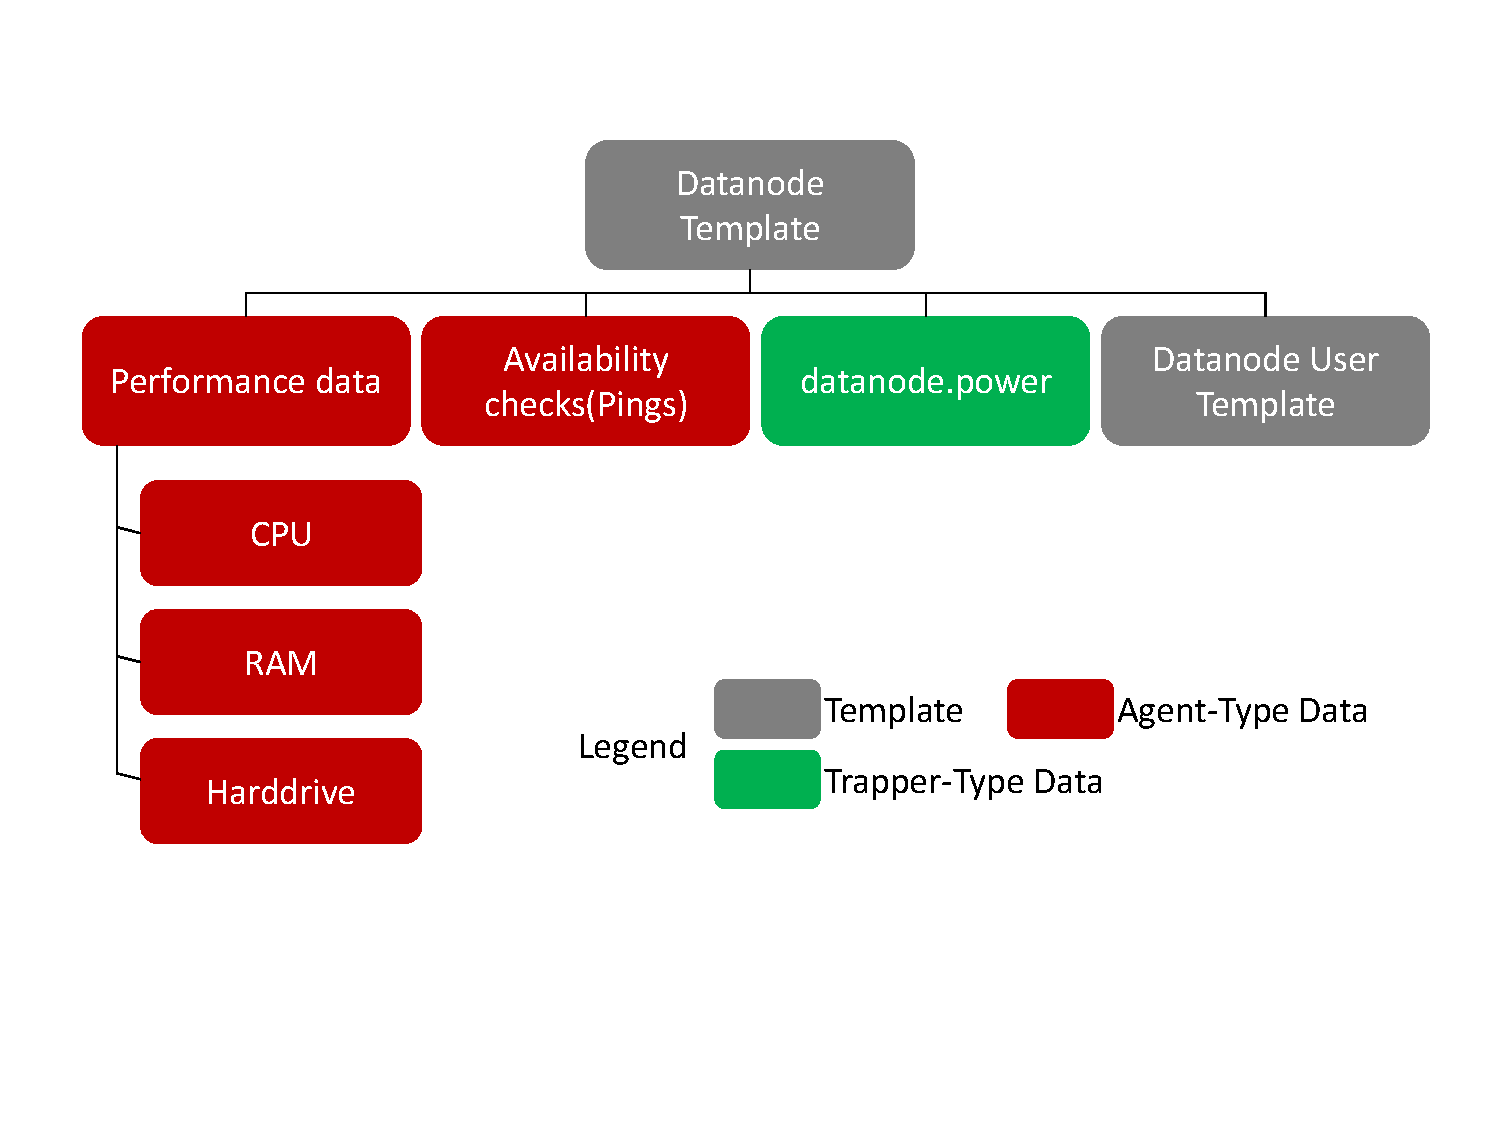
\includegraphics[width=0.5\textwidth]{img/ZabbixDatanodeTemp} 

\caption{Datatypes in the \textit{Zabbix Datanode Template}}
\label{zabbix_datanode_template}
\end{figure}
	The server template was named "Cit Project Datanode" as to represent the datanode of the  distributed file systems data storage node. Within this template were items added from the \textit{Zabbix agent} library to collect data on the monitored datanode shown in black in  figure \ref{zabbix_datanode_template}. These items were mostly \textit{Zabbix agent} items to ease the collection of system load information data. The collected data were for example heartbeat pings to ensure the corresponding datanode can still be reached and did not disconnect or crash or CPU load distributions and allocated memory to monitor the overall load on the datanode for future analysis or optimized distributions of workloads among the utilized servers and many more load or simple check data types. For the purpose of collecting such data in an efficient manner it was chosen to use the \textit{Zabbix agent} rather than trying to collect and send all these information by our own. The only manually collected and sent data field as a trapper type item was the "datanode.power" which represented the current voltage consumption for the corresponding datanode shown in light grey in figure \ref{zabbix_datanode_template}. This data was essential for the further analysis and calculations and as such was key data in the project.
\begin{figure}[ht]
\centering
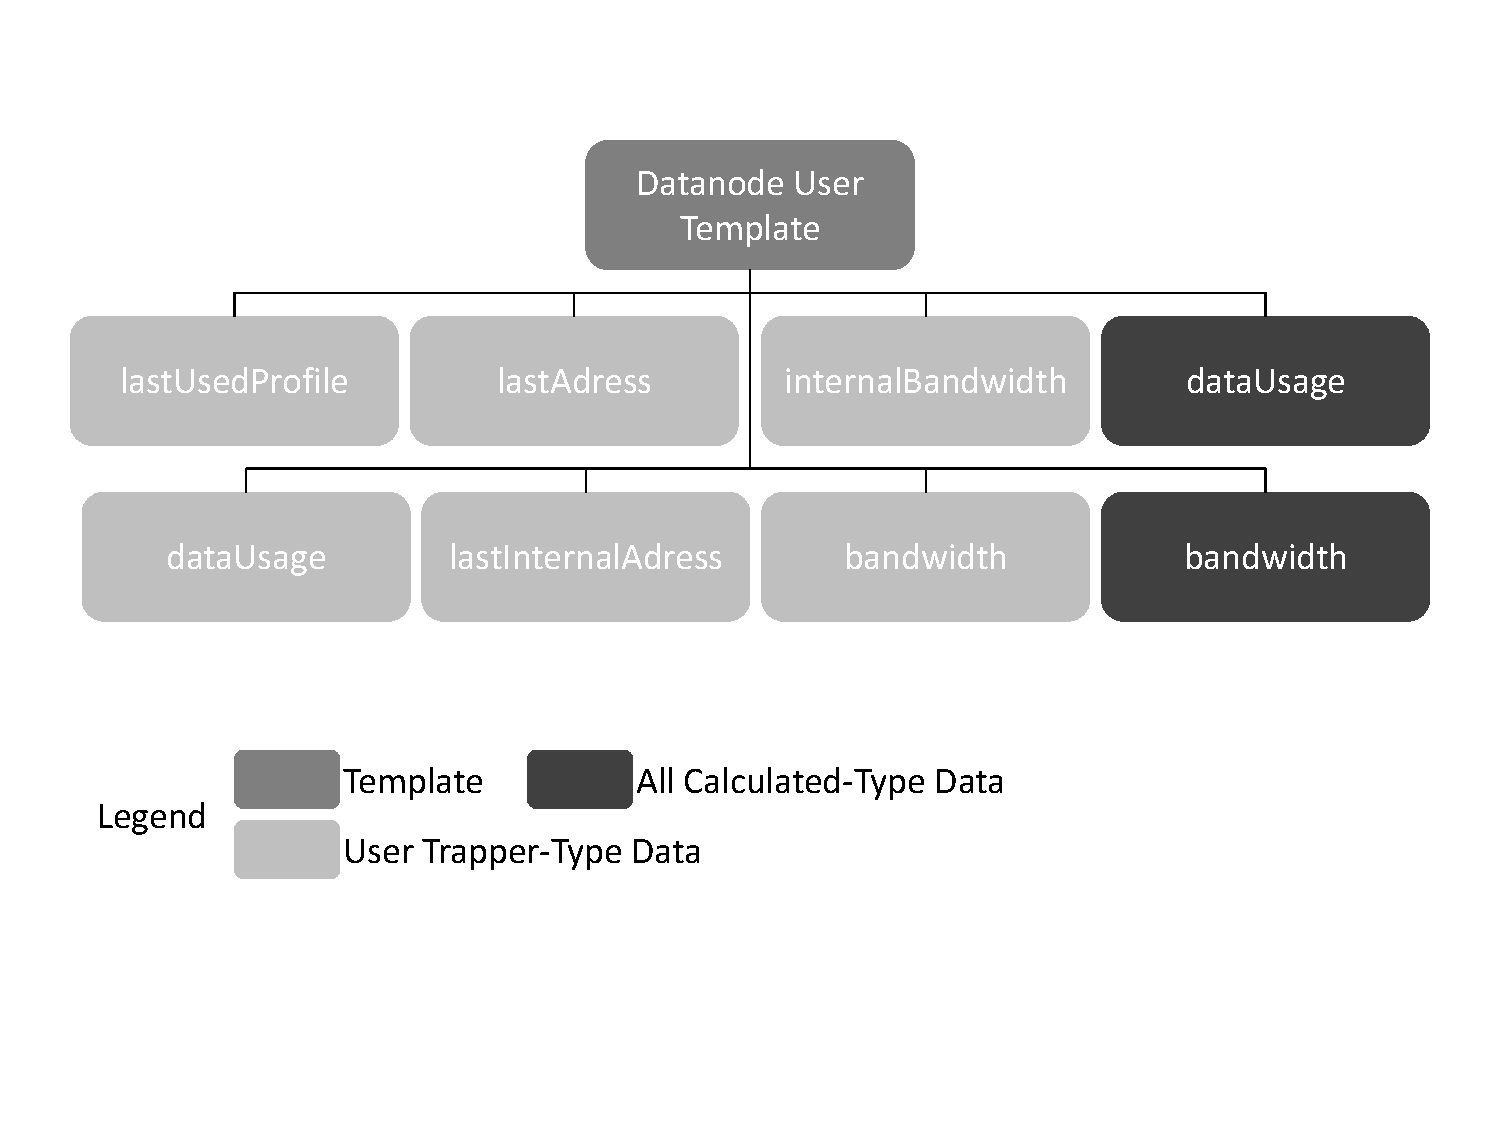
\includegraphics[width=0.5\textwidth]{img/ZabbixUserTemp} 

\caption{Datatypes in the \textit{Zabbix User Template}}
\label{zabbix_user_template}
\end{figure}	
	The user template was named "Cit Project Datanode Users" as to represent all the necessary data items for user interaction on the system and assigned to the "Cit Project Datanode" template, shown as part of the Datanode Template in figure \ref{zabbix_datanode_template}, to allow the assignment of all necessary items to every datanode representation within \textit{Zabbix} with a single template. Every user is represented through items shown in figure \ref{zabbix_user_template}, like "user.username.lastUsedProfile", "user.username.lastInternalAdress", "user.username.lastAdress", "user.username.internalBandwidth", "user.username.bandwidth" and "user.username.dataUsage". The item "user.username.lastUsedProfile" is necessary for the reporting to differentiate when the user used which kind of pricing profiles when he accessed the system. This way it is possible to calculate more precisely and fair how much expenses incurred from the users access. The items "user.username.lastInternalAdress" and "user.username.lastAdress" are for identifying the user communication stream in SDN flows to assign the resulting traffic to the right user. This is necessary since the user name information is only given once on the request to mount the distributed file system. The item "user.username.bandwidth" is representing the traffic from outside, like for example from his home, caused by the users' actions on the file system, like downloading or uploading of files. The item "user.username.internalBandwidth" however references to the traffic caused by the user which resulted from communication between the file systems data nodes for synchronization or replication of files the user had changed or created. Thus a sum of "user.username.bandwidth" and "user.username.internalBandwidth" would total the overall traffic caused by the user. Both items could be used to calculate the incurred costs from the users' activity on a single datanode. The last user item "user.username.dataUsage" is representing the allocated space on the file systems by the users' directories and files. This item is invaluable to determine the costs for the allocated space for when the user is not actively accessing the file system. All these user items are configured as trapper types to let Zabbix know that these items are being sent manually and it has to simply parse the information when it arrives. However there are two more user items, which are not specific to a single user, but rather to all users together. These are the two calculated items "user.all.dataUsage" and "user.all.bandwidth", shown in dark grey in figure \ref{zabbix_user_template}. These are as the names imply the summations of the last values of the items "user.username.dataUsage" and "user.username.bandwidth" as to give a comparative value for the total allocated space and caused traffic by all users and a  way to calculate the partial incurred traffic costs by a single user compared to the overall traffic.
	The \textit{Zabbix server} however received his very own selection of templates from a wide range of predesigned templates within \textit{Zabbix}. These templates had not only just regular server load specific data types, but also a great number of items to better monitor \textit{Zabbix} functionality and load.
\begin{figure}[ht]
\centering
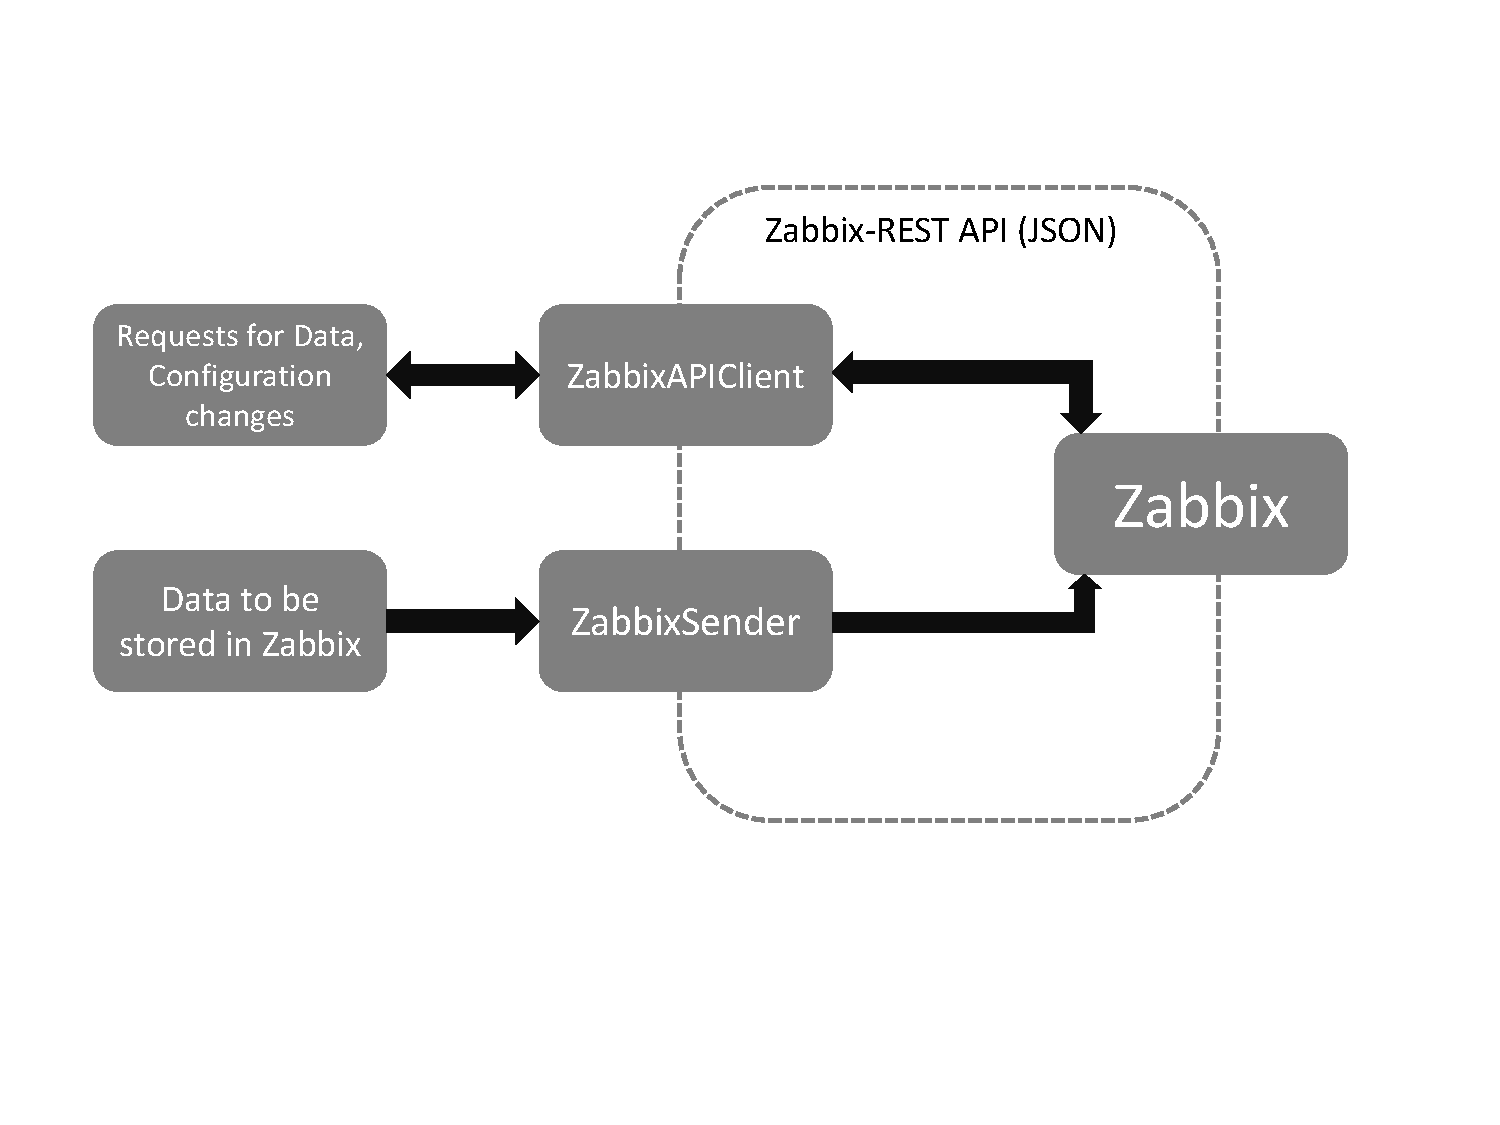
\includegraphics[width=0.5\textwidth]{img/ZabbixApiSender} 

\caption{\textit{Zabbix} Communication Interface}
\label{zabbix_api_sender}
\end{figure}
	It was decided to create a unified interface for the communication with \textit{Zabbix}. This was further split into two, the "ZabbixSender" and the "ZabbixAPIClient" as can be seen in figure \ref{zabbix_api_sender}. The "ZabbixSender" main task was to send trapper type data to \textit{Zabbix}. The use of the command line prompt \textit{zabbix\_sender} from \textit{Zabbix} was canceled as the use from a JAVA program environment forked a new thread on every send just to execute the command line. This was deemed not efficient and further the \textit{zabbix\_sender} required a library installation. It became obsolete as a method was found for packaging data into a JSON package and sending it directly to \textit{Zabbix} from a JAVA program environment. Furthermore the "ZabbixSender" was set up as a static class which is working itself through a list of queued data transfers to \textit{Zabbix}. The "ZabbixSender" is used as a one-way communication interface. The "ZabbixAPIClient" was created as a means of retrieving data from \textit{Zabbix} for example for analysis or to change the configuration of \textit{Zabbix}. Thus the "ZabbixAPIClient" housed among many the methods for data history retrieval, creating and deleting user items in the "Cit Project Datanode Users" template and the most important of them all the method for authenticating. "ZabbixAPIClient" was also set up as a static class to be continuously referenced and called but to be created only once. Both the "ZabbixSender" and the "ZabbixAPIClient" communicate with \textit{Zabbix} using its REST API interface by sending remote procedure calls in the form of JSON packages back and forth.
The listing \ref{zabcode1} is an example of such a JSON package.
\begin{lstlisting}[language=json_sw,caption={JSON authentication request\cite{zab3}},captionpos=b,numbers=left,label=zabcode1]
{
    "jsonrpc": "2.0",
    "method": "user.login",
    "params": {
        "user": "Admin",
        "password": "zabbix"
    },
    "id": 1
}\end{lstlisting} 
	This is an example of the JSON remote procedure call of the method "user.login" sent to \textit{Zabbix}. The field "id" is used to differentiate between calls to assign received results in the right way. The field "jsonrpc" simply gives the version of the JSON remote procedure calls. The field "params" holds all the information which is required for the method. In this case the only parameters are login information. For other methods the parameters can be item ids, value or item names to be searched or filtered, whole definitions of new items or hosts for item or host creation, updated formulas for calculations or graph items for graphs, flags or database expressions and many more. The JSON request after being constructed is then put into the body of an http client post with a modified header so that the request would be received correctly and then sent to \textit{Zabbix}. If \textit{Zabbix} receives the JSON package and the formatting was correct, the method existed and the parameters were fitting the method, then \textit{Zabbix} would return the result packaged in another JSON package like the example in listing \ref{zabcode2} for the JSON remote procedure call from listing \ref{zabcode1}.
	\begin{lstlisting}[language=json_sw,caption={JSON authentication response\cite{zab3}},captionpos=b,numbers=left,label=zabcode2]
{
    "jsonrpc": "2.0",
    "result": "0424bd59b807674191e7d77572075f33",
    "id": 1
}
\end{lstlisting}
	As it can be seen this result yielded just a long authentication token which in turn is necessary as another field next to "jsonrpc", "params" or "method" for many other methods, since they are requiring a certain level of rights \cite{zab3}. Thus this authentication token can be used instead of sending the login data every single time and thus creating a risk of them being compromised.
	A great number of configuration definitions like item names, template names, Zabbix login information, Zabbix URL and ports, are stored for flexibility and ease of modifications in the "ZabbixParams" class. This class stores the configuration information of Zabbix to keep the "ZabbixSender" and the "ZabbixAPIClient" free of hard-coded names.
\subsubsection{Conclusion}
	Zabbix as a monitor fulfils the requirements and it is possible to realize some of the goals, like full data model representation, creation of communication interfaces with Zabbix, visualization of great number of data types, functioning triggers, a plethora of server load specific data types, successful identification of user traffic using the IP address. However, there are spots where Zabbix does not shine as much as it would be desired. For instance, calculated items creation in the web front end only works if the formula is not empty, however through the REST API it is possible to empty it altogether, making one wonder why the web front end forbids doing so. Furthermore calculated items are prone of becoming unsupported thus being disabled for a certain span of time if some of the fields in the formula of the calculated item have no values. In general the REST API, despite its usefulness, has the tendency to result in hard to overview program code not mentioning the quite picky habits of Zabbix to which parameters it wants to succeed the remote procedure call execution. Another though albeit really small issue is with the visualization of trapper data in graphs. If the graph received some data after a longer time span it simply connects the previous value with the new one even if the data in between could have been zero but it is not deemed necessary to send a few zeros.
	All in all Zabbix does its job although with some ups and downs. It is truly hard to say whether Zabbix is or is not a well suited choice without having it undergo a test in a more or less realistic environment with dozen or even hundred of servers with a great number of users to see if Zabbix actually can run stable without being overloaded. Only such a long term observation could yield insight into the trending of data or possible energy conservation perhaps even the knowledge on how to reiterate the data model or proof for reconsideration of the choice on Zabbix. Such information is hard to discover about the project as a whole in its current state as the testing environment was quite small and for an endeavor of such big scale insufficient.

\section{Outlook}

TESTTEST

\section{Conclusion}
The conclusion goes here.



\appendices
\section{Proof of the First Zonklar Equation}
Appendix one text goes here.

\section{}
Appendix two text goes here.


% use section* for acknowledgement
\section*{Acknowledgment}
The authors would like to thank...
\ifCLASSOPTIONcaptionsoff
  \newpage
\fi


\bibliography{bib/bibliography}{}
\bibliographystyle{plain}

\end{document}


